\newpage
\def\thoigian{90}%--Thời gian
\de{Đề số 2}{Chương VI. Xác suất}

\begin{center}
	\textbf{PHẦN 1 - CÂU TRẮC NGHIỆM BỐN PHƯƠNG ÁN}
\end{center}
\Opensolutionfile{ans}[ans/ans-TN-ONTAPCHUONG6-DE2]
%Câu 1- Xác suất có điều kiện
\begin{ex}%[2D6N1-2]%[Dự án D - đợt 4 NH24-25- Hieu Hieu Minh Minh]
	Cho hai biến cố $A$ và $B$ cùng liên quan đến một phép thử. Biết $\mathrm{P}(A) = 0{,}6$; $\mathrm{P}(B) = 0{,}7$; $\mathrm{P}(A \cap B) = 0{,}3$. Xác suất $\mathrm{P}(A \mid B)$ bằng bao nhiêu?
	\choice
	{$\dfrac{1}{7}$}
	{\True $\dfrac{3}{7}$}
	{$\dfrac{6}{7}$}
	{$\dfrac{1}{2}$}
	\loigiai{
		Ta có $\mathrm{P}(A \mid B) = \dfrac{\mathrm{P}(A \cap B)}{\mathrm{P}(B)} = \dfrac{0{,}3}{0{,}7} = \dfrac{3}{7}$.
	}
\end{ex}
%Câu 2 - Xác suất có điều kiện
\begin{ex}%[2D6N1-1]%[Dự án D - đợt 4 NH24-25- Hieu Hieu Minh Minh]
	Cho hai biến cố $A$ và $B$ bất kì, với $\mathrm{P}(B) > 0$. Khẳng định nào sau đây là đúng?
	\choice
	{$\mathrm{P}(A|B) = \dfrac{\mathrm{P}(A \cup B)}{\mathrm{P}(B)}$}
	{$\mathrm{P}(A|B) = \dfrac{\mathrm{P}(A) \cdot \mathrm{P}(B)}{\mathrm{P}(B)}$}
	{\True $\mathrm{P}(A|B) = \dfrac{\mathrm{P}(AB)}{\mathrm{P}(B)}$}
	{$\mathrm{P}(A|B) = \dfrac{\mathrm{P}(A) + \mathrm{P}(B)}{\mathrm{P}(B)}$}
	\loigiai
	{Công thức xác suất có điều kiện là $\mathrm{P}(A|B) = \dfrac{\mathrm{P}(AB)}{\mathrm{P}(B)}$.
	}
\end{ex}
%Câu 3 - Xác suất có điều kiện
\begin{ex}%[2D6H1-3]%[Dự án D - đợt 4 NH24-25- Hieu Hieu Minh Minh]
	Trong một cuộc khảo sát trên một nhóm gồm $50$ học sinh chơi cầu lông, thu được kết quả như bảng số liệu sau
	\begin{center}
		\begin{tikzpicture}
			\path 
			(0,0) coordinate (O)
			(2.8,-1) coordinate (A) node [above]{$\text{ Tay thuận}$}
			(1,-1) coordinate (B) node [below] {$\text{Giới tính}$}
			(2,-2.5) coordinate (C) node {$\text{Nam}$}
			(2,-3.5) coordinate (D) node {$\text{Nữ}$}
			(5,-1) coordinate (E) node {$\text{Tay trái}$}
			(7,-1) coordinate (F) node {$\text{Tay phải}$}
			(5,-2.5) coordinate (G) node  {$5$}
			(7,-2.5) coordinate (H) node {$32$}
			(5,-3.5) coordinate (I) node {$2$}
			(7,-3.5) coordinate (K) node {$11$}
			;
			\draw (O) rectangle (8,-4);
			\draw (4,0)--(4,-4) (6,0)--(6,-4) (0,-2)--(8,-2) (0,-3)--(8,-3) (0,0)--(4,-2)
			;
		\end{tikzpicture}
	\end{center}
	Chọn ngẫu nhiên một học sinh trong nhóm này. Tính xác suất để học sinh đươc chọn là nam, biết học sinh đó thuận tay phải.
	\choice
	{\True$\dfrac{32}{43}$}
	{$\dfrac{32}{37}$}
	{$\dfrac{16}{25}$}
	{$\dfrac{11}{4}$} 
	\loigiai{
		Gọi biến cố $A\colon$\lq\lq Học sinh được chọn là nam\rq\rq.\\
		Gọi biến cố $B\colon$ \lq\lq Học sinh thuận tay phải\rq\rq.\\
		Ta cần tính $\mathrm{P}(A|B)=\dfrac{32}{32+11}=\dfrac{32}{43}$.
	}
\end{ex}
%Câu 4 - Xác suất có điều kiện
\begin{ex}%[2D6H1-1]%[Dự án D - đợt 4 NH24-25- Hieu Hieu Minh Minh]
	Cho hai biến cố $A$, $B$ của cùng một phép thử thỏa mãn $\mathrm{P}(A) = 0{,}5$; $\mathrm{P}(B) = 0{,}6$; $\mathrm{P}(A \cup B) = 0{,}7$. Khi đó $\mathrm{P}(B|A)$ bằng
	\choice
	{$\dfrac{2}{3}$}
	{$0{,}6$}
	{\True $0{,}8$}
	{$0{,}5$}
	\loigiai{
		Ta có công thức
		\[
		\mathrm{P}(A \cup B) = \mathrm{P}(A) + \mathrm{P}(B) - \mathrm{P}(A \cap B) \Rightarrow 0{,}7 = 0{,}5 + 0{,}6 - \mathrm{P}(A \cap B).
		\]
		Suy ra $\mathrm{P}(A \cap B) = 0{,}4$.\\
		Do đó
		\[\mathrm{P}(B|A) = \dfrac{\mathrm{P}(A \cap B)}{\mathrm{P}(A)} = \dfrac{0{,}4}{0{,}5} = \dfrac{4}{5}=0{,}8.\]
	}
\end{ex}
%Câu 5 - Xác suất có điều kiện
\begin{ex}%[2D6N2-1]%[Dự án D - đợt 4 NH24-25- Hieu Hieu Minh Minh]
	Cho $A$ và $B$ là hai biến cố bất kì, với $0<\mathrm{P}(B)<1$. Khi đó
	\choice
	{$\mathrm{P}(B \mid A)=\dfrac{\mathrm{P}(A B)}{\mathrm{P}(B)}$}
	{\True $\mathrm{P}(A \mid B)=\dfrac{\mathrm{P}(A B)}{\mathrm{P}(B)}$}
	{$\mathrm{P}(A \mid B)=\dfrac{\mathrm{P}(B)}{\mathrm{P}(A B)}$}
	{$\mathrm{P}(B \mid A)=\dfrac{\mathrm{P}(A B)}{\mathrm{P}(\overline{B})}$}
	\loigiai{Cho $A$ và $B$ là hai biến cố bất kì, với $0<\mathrm{P}(B)<1$.\\ Khi đó $\mathrm{P}(A \mid B)=\dfrac{\mathrm{P}(A B)}{\mathrm{P}(B)}$.
	}
\end{ex}
%Câu 6 - Xác suất có điều kiện
\begin{ex}%[2D6H1-2]%[Dự án D - đợt 4 NH24-25- Hieu Hieu Minh Minh]
	Gieo con xúc xắc cân đối, đồng chất và được gieo $1$ lần. Gọi $A$ là biến cố \lq\lq xuất hiện mặt $2$ chấm\rq\rq, $B$ là biến cố \lq\lq xuất hiện mặt chẵn chấm\rq\rq. Xác suất $\mathrm{P}\left(A\mid B\right)$ là
	\choice
	{$\dfrac{1}{2}$}
	{\True $\dfrac{1}{3}$}
	{$\dfrac{2}{3}$}
	{$\dfrac{1}{6}$}
	\loigiai{
		Gieo con xúc xắc $1$ lần thì không gian mẫu là $\Omega=\left\lbrace1;2;3;4;5;6 \right\rbrace$.\\
		Số phần tử của không gian mẫu là $n\left(\Omega\right)=6$.\\
		Ta có biến cố $B$ (xuất hiện mặt chẵn) là $B=\left\lbrace2;4;6\right\rbrace$.\\
		Số phần tử của biến cố $B$ là $n\left(B\right)=3$.\\
		Xác suất của $B$ là $\mathrm{P}\left(B\right)=\dfrac{n\left(B\right)}{n\left(\Omega\right)}=\dfrac{3}{6}=\dfrac{1}{2}$.\\
		Ta có biến cố giao $A \cap B$ (xuất hiện mặt $2$ chấm và là mặt chẵn) là $A \cap B = \left\lbrace 2\right\rbrace$.\\
		Số phần tử của biến cố $A \cap B$ là $n\left(A \cap B\right)=1$.\\
		Xác suất của $A \cap B$ là $\mathrm{P}\left(A \cap B\right)=\dfrac{n\left(A \cap B\right)}{n\left(\Omega\right)}=\dfrac{1}{6}$.\\
		Áp dụng công thức xác suất có điều kiện ta có
		$\mathrm{P}\left(A\mid B\right)=\dfrac{\mathrm{P}\left(A \cap B\right)}{\mathrm{P}\left(B\right)}=\dfrac{\dfrac{1}{6}}{\dfrac{1}{2}}
		=\dfrac{1}{3}$.
	}
\end{ex}
%Câu 7 - Xác suất toàn phần và công thức Bayes
\begin{ex}%[2D6H2-2]%[Dự án D - đợt 4 NH24-25- Hieu Hieu Minh Minh]
	Cho $2$ biến cố $A$ và $B$. Biết $\mathrm{P}(A\mid B)=0{,}8$; $\mathrm{P}(A\mid \overline{B})=0{,}3$; $\mathrm{P}(B)=0{,}4$. Giá trị $\mathrm{P}(A)$ bằng
	\choice
	{$0{,}04$}
	{\True $0{,}5$}
	{$0{,}1$}
	{$0{,}55$}
	\loigiai{Ta có $\mathrm{P}(\overline{B})=1-\mathrm{P}(B)=0{,}6.$\\ 
		Áp dụng công thức xác suất toàn phần ta có $$\mathrm{P}(A)=\mathrm{P}(A\mid B)\cdot \mathrm{P}(B)+\mathrm{P}(A\mid \overline{B})\cdot \mathrm{P}(\overline{B})=0{,}8\cdot 0{,}4+0{,}3\cdot 0{,}6=0{,}5.$$}
	
\end{ex}
%Câu 8 - Xác suất toàn phần và công thức Bayes
\begin{ex}%[2D6N2-1]%[Dự án D - đợt 4 NH24-25- Hieu Hieu Minh Minh]
	Cho $A$, $B$ là các biến cố của một phép thử $T.$ Biết rằng $P\left( B \right)>0,$ xác suất của biến cố $A$ với điều kiện biến cố $B$ đã xảy ra được tính theo công thức nào sau đây?
	\choice
	{$P\left( \left. A \right|B \right)=\dfrac{P\left( A \right)}{P\left( B \right)}$}
	{\True $P\left( \left. A \right|B \right)=\dfrac{P\left( A \right).P\left( \left. B \right|A \right)}{P\left( B \right)}$}
	{$P\left( \left. A \right|B \right)=\dfrac{P\left( B \right).P\left( \left. B \right|A \right)}{P\left( A \right)}$}
	{$P\left( \left. A \right|B \right)=\dfrac{P\left( B \right)}{P\left( A \right)}$}
	\loigiai{
		Theo công thức Bayes, ta có $P\left( \left. A \right|B \right)=\dfrac{P\left( A \right).P\left( \left. B \right|A \right)}{P\left( B \right)}.$
	}
	\end{ex}
%Câu 9 - Xác suất toàn phần và công thức Bayes
\begin{ex}%[2D6H2-2]%[Dự án D - đợt 4 NH24-25- Hieu Hieu Minh Minh]
	Cho $A$, $B$ là hai biến cố của một phép thử có sơ đồ hình cây như sau
	\begin{center}
		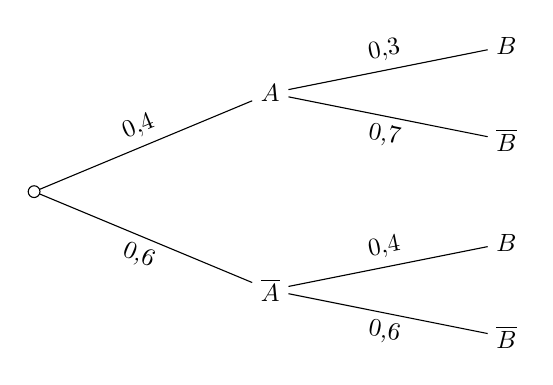
\begin{tikzpicture}[
			grow=right,
			level distance=3cm,
			sibling distance=2.5cm,
			level 2/.style={sibling distance=1.2cm},
			every node/.style={scale=0.9}
			]
			\node [draw, circle, scale=0.5] {}
			child { node{$\overline{A}$}
				child { node{$\overline{B}$}
					edge from parent[sloped] node[below] {$0{,}6$}
				}
				child { node{$B$}
					edge from parent[sloped] node[above] {$0{,}4$}
				}
				edge from parent[sloped] node[below] {$0{,}6$}
			}
			child { node{$A$}
				child { node{$\overline{B}$}
					edge from parent[sloped] node[below] {$0{,}7$}
				}
				child { node{$B$}
					edge from parent[sloped] node[above] {$0{,}3$}
				}
				edge from parent[sloped] node[above] {$0{,}4$}
			};
		\end{tikzpicture}
	\end{center}
	Xác suất của biến cố $B$ là
	\choice
	{$\mathrm{P}(B)=0{,}4\cdot0{,}3$}
	{$\mathrm{P}(B)=0{,}6\cdot0{,}4$}
	{\True $\mathrm{P}(B)=0{,}4\cdot0{,}3+0{,}6\cdot0{,}4$}
	{$\mathrm{P}(B)=0{,}4\cdot0{,}3-0{,}6\cdot0{,}4$}
	\loigiai
	{Xác suất để $B$ xảy ra là \\
		$\mathrm{P}(B) = \mathrm{P}(A).\mathrm{P}(B|A) + \mathrm{P}(\overline{A}).\mathrm{P}(B|\overline{A}) = 0{,}4 \cdot 0{,}3 + 0{,}6 \cdot 0{,}4 = 0{,}12 + 0{,}24 = 0{,}36$.
	}
\end{ex}
%Câu 10 - Xác suất toàn phần và công thức Bayes
\begin{ex}%[2D6N2-1]%[Dự án D - đợt 4 NH24-25- Hieu Hieu Minh Minh]
	Cho hai biến cố $A$ và $B$ với $0<\mathrm{P}\left(B\right)<1$. Khẳng định nào sau đây là đúng?
	\choice
	{\True $\mathrm{P}\left(A\right)=\mathrm{P}\left(B\right)\cdot\mathrm{P}\left(A\mid B\right)+\mathrm{P}\left(\overline{B}\right)\cdot\mathrm{P}\left(A\mid\overline{B}\right)$}
	{$\mathrm{P}\left(A\right)=\mathrm{P}\left(A\right)\cdot \mathrm{P}\left(A\mid B\right)+\mathrm{P}\left(\overline{A}\right)\cdot \mathrm{P}\left(A\mid \overline{B}\right)$}
	{$\mathrm{P}\left(A\right)=\mathrm{P}\left(B\right)\cdot\mathrm{P}\left(A\mid\overline{B}\right)+\mathrm{P}\left(\overline{B}\right)\cdot \mathrm{P}\left(A\mid B\right)$}
	{$\mathrm{P}\left(A\right)=\mathrm{P}\left(B\right)\cdot\mathrm{P}\left(A\mid B\right)-\mathrm{P}\left(\overline{B}\right)\cdot\mathrm{P}\left(A\mid \overline{B}\right)$}
	\loigiai{
		Theo công thức xác suất toàn phần, ta có $\mathrm{P}\left(A\right)=\mathrm{P}\left(B\right)\cdot \mathrm{P}\left(A\mid B\right)+\mathrm{P}\left(\overline{B}\right)\cdot \mathrm{P}\left(A\mid\overline{B}\right)$.
	}
\end{ex}
%Câu 11 - Xác suất toàn phần và công thức Bayes
\begin{ex}%[2D6H2-2]%[Dự án D - đợt 4 NH24-25- Hieu Hieu Minh Minh]
	Một cuộc khảo sát, có $200$ người tham gia, trong đó có $120$ người sử dụng smartphone và $80$ người sử dụng máy tính bảng. Trong số những người sử dụng smartphone, $70\%$ có sử dụng mạng xã hội. Trong số những người sử dụng máy tính bảng, $40\%$ có sử dụng mạng xã hội. Một người được chọn ngẫu nhiên từ $200$ người tham gia khảo sát. Xác suất để người đó là người sử dụng smartphone, biết rằng người đó đã sử dụng mạng xã hội bằng
	\choice
	{$\dfrac{3}{7}$}
	{\True $\dfrac{21}{29}$}
	{$\dfrac{29}{50}$}
	{$\dfrac{8}{29}$}
	\loigiai{		
		Gọi $A$ là biến cố \lq\lq người sử dụng smartphone\rq\rq, $B$ là biến cố \lq\lq người dùng mạng xã hội\rq\rq.\\
		Ta có sơ đồ cây minh họa các dữ kiện bài toán
		\begin{center}
			\begin{tikzpicture}[
				grow=right,
				level distance=3cm,
				sibling distance=2.5cm,
				level 2/.style={sibling distance=1.2cm},
				every node/.style={scale=0.9}
				]
				\node [draw, circle, scale=0.5] {}
				child { node{$\overline{A}$}
					child { node{$\overline{B}$}
						edge from parent[sloped] node[below] {?}
					}
					child { node{$B$}
						edge from parent[sloped] node[above] {$40\%$}
					}
					edge from parent[sloped] node[below] {$\dfrac{80}{200}$}
				}
				child { node{$A$}
					child { node{$\overline{B}$}
						edge from parent[sloped] node[below] {?}
					}
					child { node{$B$}
						edge from parent[sloped] node[above] {$70\%$}
					}
					edge from parent[sloped] node[above] {$\dfrac{120}{200}$}
				};
			\end{tikzpicture}
		\end{center}
		Suy ra, $A|B$ là biến cố \lq\lq người đó là người sử dụng smartphone, biết rằng người đó đã sử dụng mạng xã hội\rq\rq.\\
		Khi đó $\mathrm{P}(A) = \dfrac{120}{200}=0{,}6$; $\mathrm{P}\left(B|A\right) = 70\%=0{,}7$; $\mathrm{P}\left(B|\overline{A}\right) = 40\%=0{,}4$.\\
		Ta có $\mathrm{P}\left(\overline{A}\right) = 1-0{,}6=0{,}4$.\\
		Ta có $\mathrm{P}(B) = \mathrm{P}(A)\cdot\mathrm{P}\left(B|A\right) + \mathrm{P}\left(\overline{A}\right) \cdot\mathrm{P}\left(B|\overline{A}\right)=0{,}6 \cdot 0{,}7 + 0{,}4 \cdot 0{,}4 = 0{,}42 + 0{,}16 = 0{,}58$.\\
		Vậy $\mathrm{P}\left(A|B\right) = \dfrac{\mathrm{P}(AB)}{\mathrm{P}(B)} = \dfrac{0{,}6 \cdot 0{,}7}{0{,}58} = \dfrac{0{,}42}{0{,}58} = \dfrac{21}{29}$.\\
	}
\end{ex}
%Câu 12 - Xác suất toàn phần và công thức Bayes
\begin{ex}%[2D6H2-3]%[Dự án D - đợt 4 NH24-25- Hieu Hieu Minh Minh]
	Cho hai biến cố $A$, $B$ thoả mãn $P\left( A \right)=0{,}4$; $P\left( B \right)=0{,}3$; $P\left( A\mid B \right)=0{,}25$. Khi đó, $P\left( B\mid A \right)$ bằng
	\choice
	{\True $0{,}1875$}
	{$0{,}48$}
	{$0{,}333$}
	{$0{,}95$}
	\loigiai{
		Theo công thức Bayes, ta có $P\left( B\mid A \right)=\dfrac{P\left( B \right) \cdot P\left( A\mid B \right)}{P\left( A \right)}=\dfrac{0{,}3 \cdot 0{,}25}{0{,}4}=0{,}1875$.
	}
\end{ex}

\Closesolutionfile{ans}
%\begin{center}
%	\textbf{ĐÁP ÁN}
%	\inputansbox{10}{ans/ans}	
%\end{center}

\begin{center}
	\textbf{PHẦN 2 - CÂU TRẮC NGHIỆM ĐÚNG SAI}
\end{center}
\setcounter{ex}{0}
\Opensolutionfile{ans}[ans/answer-DS-ONTAPCHUONG6-DE2]
%Câu 1%
\begin{ex}%[2D6H1-2]%[Dự án D - đợt 4 NH24-25- Hieu Hieu Minh Minh]
	Một lớp học có $40$ học sinh, trong đó có $27$ học sinh nam và $13$ học sinh nữ. Thống kê điểm kiểm tra cuối học kì I, lớp có $18$ em đạt điểm trung bình trở lên, trong đó có $8$ học sinh nam và $10$ học sinh nữ. Chọn ngẫu nhiên $1$ học sinh trong lớp.
	\choiceTF
	{\True Xác suất học sinh được chọn là học sinh nam bằng $0{,}675$}
	{Xác suất học sinh được chọn là học sinh nữ bằng $0{,}315$}
	{\True Xác suất học sinh được chọn là học sinh nam và đạt điểm trung bình trở lên bằng $0{,}2$}
	{Biết rằng học sinh được chọn là nữ, xác suất học sinh đó không đạt điểm trung bình là $\dfrac{19}{27}$}
	\loigiai
	{Ta có bảng mô tả các dữ kiện của bài toán như sau
		\begin{center}
			\begin{tikzpicture}
				\def\cw{3}
				\def\rh{1}
				\draw (0,0) rectangle (\cw*4,-\rh*4);
				\foreach \i in {1,2,3} {
					\draw (\cw*\i, 0) -- (\cw*\i, -\rh*4);
				}
				\foreach \j in {1,2,3} {
					\draw (0, -\rh*\j) -- (\cw*4, -\rh*\j);
				}
				\draw (0,0) -- (\cw,-\rh);
				\node[align=center] at (0.7, -0.7) {GT};
				\node[align=center] at (2.3, -0.3) {Điểm};
				\node at (\cw*1.5, -0.5) {TB trở lên};
				\node at (\cw*2.5, -0.5) {Dưới TB};
				\node at (\cw*3.5, -0.5) {Tổng};
				\node at (0.7, -\rh*1.5) {Nam};
				\node at (0.7, -\rh*2.5) {Nữ};
				\node at (0.7, -\rh*3.5) {Cộng};
				\node at (\cw*1.5, -\rh*1.5) {$8$};
				\node at (\cw*2.5, -\rh*1.5) {$?$};
				\node at (\cw*3.5, -\rh*1.5) {$27$};
				\node at (\cw*1.5, -\rh*2.5) {$10$};
				\node at (\cw*2.5, -\rh*2.5) {$?$};
				\node at (\cw*3.5, -\rh*2.5) {$13$};
				\node at (\cw*1.5, -\rh*3.5) {$18$};
				\node at (\cw*2.5, -\rh*3.5) {$?$};
				\node at (\cw*3.5, -\rh*3.5) {$40$};
			\end{tikzpicture}
		\end{center}
		Gọi $A\colon$\lq\lq học sinh được chọn là nam\rq\rq, $B\colon$\lq\lq học sinh được chọn đạt điểm trung bình trở lên\rq\rq.\\
		Khi đó $\overline{A}$ là biến cố \lq\lq học sinh được chọn là nữ\rq\rq, $\overline{B}$ là biến cố \lq\lq học sinh được chọn có điểm dưới trung bình\rq\rq.\\
		Ta có $n(\Omega)=40$.\\
		\begin{itemchoice}
			\itemch 
			$n(A)=27\Rightarrow \mathrm{P}(A) = \dfrac{27}{40} = 0{,}675$.
			\itemch 
			$n(B)=13\Rightarrow \mathrm{P}(A) = \dfrac{13}{40} = 0{,}325$.
			\itemch 
			$n(A\cap B)=8\Rightarrow \mathrm{P}(A) = \dfrac{8}{40} = 0{,}2$.
			\itemch 
			$n\left(\overline{A}\cap \overline{B}\right)=13-10=3$, $n\left(\overline{A}\right)=13$.\\
			Suy ra $\mathrm{P}\left(\overline{B}| \overline{A}\right) =\dfrac{n\left(\overline{A}\cap \overline{B}\right)}{n\left(\overline{A}\right)} =\dfrac{3}{13}$.
		\end{itemchoice}
	}
\end{ex}
%Câu 2%
\begin{ex}%[2D6V2-4]%[Dự án D - đợt 4 NH24-25- Hieu Hieu Minh Minh]
	Trong kỳ kiểm tra môn Toán của một trường THPT có $400$ học sinh tham gia, trong đó có $180$ học sinh nam và $220$ học sinh nữ. Khi công bố kết quả kỳ kiểm tra đó, tỉ lệ học sinh đạt điểm giỏi tương ứng với nam và nữ lần lượt là $25\%$ và $30\%$. Chọn ngẫu nhiên một học sinh trong số $400$ học sinh đó.\\
	Gọi $A\colon$\lq\lq Học sinh được chọn ra đạt điểm giỏi \rq\rq;\\$B\colon$\lq\lq Học sinh được chọn ra là học sinh nữ \rq\rq.
	\choiceTF
	{\True Xác suất $\mathrm{P}(B)=\dfrac{9}{20}$ và $\mathrm{P}(\overline{B})=\dfrac{11}{20}$}
	{Xác suất có điều kiện $\mathrm{P}(A \mid \overline{B})=0{,}3$}
	{\True Xác suất $\mathrm{P}(\overline{A})=0{,}7225$}
	{\True Trong số học sinh đạt điểm giỏi có $59\%$ học sinh nữ đạt điểm giỏi trong kì kiểm tra môn Toán (kết quả làm tròn đến hàng đơn vị)}
	\loigiai{
		\begin{itemchoice}
			\itemch \textbf{Đúng}.\\
			Ta có $\mathrm{P}(B) = \dfrac{220}{400}=\dfrac{11}{20}$ và $\mathrm{P}\left(\overline{B}\right) =\dfrac{180}{440}= \dfrac{9}{20}$.
			\itemch \textbf{Sai}.\\
			Xác suất có điều kiện $\mathrm{P}(A \mid \overline{B})$ là $\mathrm{P}\left(A\mid \overline{B}\right)=0{,}25$.
			\itemch \textbf{Đúng}.\\
			Áp dụng công thức xác suất toàn phần, ta có
			\[\mathrm{P}(A)= \mathrm{P}(B) \cdot \mathrm{P}\left(A \mid B\right)+\mathrm{P}\left(\overline{B}\right) \cdot \mathrm{P}\left(A \mid \overline{B}\right)= \dfrac{11}{20} \cdot 0{,}3+\dfrac{9}{20} \cdot 0{,}25=0{,}2775.\]
			Khi đó
			\[\mathrm{P}\left(\overline{A}\right)=1-\mathrm{P}(A)=1-0{,}2775=0{,}7225.\]
			\itemch \textbf{Đúng}.\\
			Trong số học sinh đạt điểm giỏi, xác suất để bạn đó là học sinh nữ là
			\[\mathrm{P}(B \mid A) =\dfrac{\mathrm{P}(B) \cdot \mathrm{P}(A \mid B)}{\mathrm{P}(A)}=\dfrac{\dfrac{11}{20} \cdot 0{,}3}{0{,}2775}=\dfrac{22}{37} \approx 59\%.\]	
		\end{itemchoice}
	}
	
\end{ex}
\Closesolutionfile{ans}
%\inputansbox[2]{2}{ans/answer.tex}

\begin{center}
\textbf{PHẦN 3 - CÂU TRẮC NGHIỆM TRẢ LỜI NGẮN}
\end{center}
\setcounter{ex}{0}
\Opensolutionfile{ans}[ans/ans-KQ-ONTAPCHUONG6-DE2]
%Câu 1%
\begin{ex}%[2D6H1-2]%[Dự án D - đợt 4 NH24-25- Hieu Hieu Minh Minh]
	Trong số $45$ hệ nhóm máu đươc ghi nhận, $ABO$ vẫn là hệ thống quan trọng nhất trong truyền máu và ghép tạng vì hầu hết mọi người trên $6$ tháng tuổi đều có kháng thể kháng $A$ hoặc kháng $B$ có ý nghĩa lâm sàng trong huyết thanh. Nhóm máu $A$ chứa kháng thể chống lại nhóm máu $B$ trong huyết thanh và ngược lại, trong khi nhóm máu $O$ không chứa kháng nguyên $A$ và kháng nguyên $B$ nhưng có cả kháng thể kháng $A$ và kháng $B$ trong huyết thanh. Hệ nhóm máu $ABO$ gồm $4$ nhóm máu là $A$, $B$, $O$ và $AB$ với tỷ lệ phân bố trong cộng đồng khác nhau ở từng chủng tộc. Ở Việt Nam, tỷ lệ này là: nhóm $O$ khoảng $45\%$, nhóm $B$ khoảng $30\%$, nhóm $A$ khoảng $20\%$ và nhóm $AB$ khoảng $5\%$. Lấy ngẫu nhiên một người cần hiến máu và một người hiến máu. Tính xác suất có thể thực hiện truyền máu (đơn vị $\%$ kết quả làm tròn đến hàng phần chục).	
	\shortans{$60{,}8$}
	\loigiai{
		Ta có
		\begin{itemize}
			\item Nhóm máu $A$ có thể truyền cho nhóm máu $A$ và $AB$.
			\item Nhóm máu $B$ có thể truyền cho nhóm máu $B$ và $AB$.
			\item Nhóm máu $O$ có thể truyền cho tất cả nhóm máu.
			\item Nhóm máu $AB$ chỉ có thể truyền cho $AB$.
		\end{itemize}
		\textbf{Trường hợp 1:} Người  hiến máu có nhóm máu $A$, khi đó người cần hiến máu phải thuộc nhóm máu $A$ hoặc $AB$.\\
		Suy ra xác suất có thể truyền máu là $20\%\cdot (20\%+5\%)=0{,}05$.\\
		\textbf{Trường hợp 2:} Người hiến máu có nhóm máu $B$, khi đó người cần hiến máu phải thuộc nhóm máu $B$ hoặc $AB$.\\
		Suy ra xác suất có thể truyền máu là $30\%\cdot (30\%+5\%)=0{,}105$.\\
		\textbf{Trường hợp 3:} Người hiến máu có nhóm máu $O$, khi đó người cần hiến máu có thể thuộc nhóm máu bất kỳ.\\
		Suy ra xác suất có thể truyền máu là $45\%=0{,}45$.\\
		\textbf{Trường hợp 4:} Người hiến máu có nhóm máu $AB$, khi đó người cần hiến máu phải thuộc nhóm máu $AB$.\\
		Suy ra xác suất có thể truyền máu là $5\%\cdot5\%=0{,}0025$.\\
		Vậy xác suất có thể truyền máu là $0{,}05+0{,}105+0{,}45+0{,}0025=0{,}6075=60{,}75\%\approx 60{,}8\%$.
	}
\end{ex}
%Câu 2%
\begin{ex}%[2D5H1-2]%[Dự án D - đợt 4 NH24-25- Hieu Hieu Minh Minh]
	Một thư viện có hai phòng riêng biệt, phòng $I$ và phòng $II$. Chọn ngẫu nhiên một cuốn sách ở thư viện đó. Biết rằng, xác suất để chọn được một cuốn sách Toán và ở phòng $I$ là $0{,}21$; xác suất để chọn được một cuốn sách Toán và ở phòng $II$ là $0{,}63$. Nếu cuốn sách được chọn là sách Toán thì xác
	suất để cuốn sách đó ở phòng $I$ bằng bao nhiêu?
	\shortans{$0{,}25$}
	\loigiai{Gọi $A\colon$ \lq \lq Cuốn sách được chọn là sách Toán \rq \rq;\\
		$B\colon$ \lq \lq Cuốn sách được chọn ở phòng $I$ \rq \rq.\\
		Vì xác suất để chọn được một cuốn sách Toán và ở phòng $I$ là $0{,}21$ nên $\mathrm{P} \left(AB \right) = 0{,}21$.\\
		Vì xác suất để chọn được một cuốn sách Toán và ở phòng $II$ là $0{,}63$ nên $\mathrm{P} \left(A\overline{B} \right) = 0{,}63$.\\
		Ta có  $\mathrm{P} \left(A \right) = \mathrm{P} \left(AB \right) +\mathrm{P} \left(A\overline{B} \right) = 0{,}21+0{,}63=0{,}84$.\\
		Nếu cuốn sách được chọn là sách Toán thì xác
		suất để cuốn sách đó ở phòng $I$ là
		$$\mathrm{P} \left(B \mid A\right) = \dfrac{\mathrm{P} \left(AB\right)}{\mathrm{P} \left(A\right)}=\dfrac{0{,}21}{0{,}84}=0{,}25.$$
	}
\end{ex}
%Câu 3%
\begin{ex}%[2D6V2-3]%[Dự án D - đợt 4 NH24-25- Hieu Hieu Minh Minh]
	Trường THPT $X$, có $20\%$ học sinh tham gia câu lạc bộ âm nhạc, trong số học sinh đó thì có $75\%$ học sinh biết chơi đàn guitar. Ngoài ra, trong số học sinh không tham gia câu lạc bộ âm nhạc có $10\%$ học sinh biết chơi đàn guitar. Chọn ngẫu nhiên $1$ học sinh của trường. Giả sử học sinh đó biết chơi đàn guitar. Xác suất để chọn được học sinh thuộc câu lạc bộ âm nhạc là bao nhiêu? (làm tròn đến hàng phần trăm).
	\shortans{$0,65$}
	\loigiai{
		Gọi $A$ là biến cố \lq\lq Học sinh tham gia CLB âm nhạc\rq\rq, ta có $\mathrm{P}(A)=0{,}2\Rightarrow \mathrm{P}(\overline{A})=1-0{,}2=0{,}8$.\\
		Gọi $G$ là biến cố \lq\lq Học sinh biết chơi đàn guitar\rq\rq, ta có $\mathrm{P}(G\mid A) = 0{,}75$; $\mathrm{P}(G\mid \overline{A}) = 0{,}1$.\\
		Xác suất để chọn được học sinh thuộc CLB âm nhạc, biết rằng học sinh đó biết chơi đàn guitar là $$\mathrm{P}(A\mid G)=\frac{ \mathrm{P}(G\mid A)\cdot \mathrm{P}(A)}{\mathrm{P}(G\mid A)\cdot \mathrm{P}(A)+\mathrm{P}(G\mid\overline{A})\cdot \mathrm{P}(\overline{A})}=\frac{0{,}75 \cdot  0{,}2}{0{,}75 \cdot  0{,}2 + 0{,}1 \cdot  0{,}8 }  = \frac{0{,}15}{0{,}15 + 0{,}08} \approx 0{,}65.$$
	}
\end{ex}
%Câu 4%
\begin{ex}%[2D6V2-3]%[Dự án D - đợt 4 NH24-25- Hieu Hieu Minh Minh]
	Một kho hàng do hai nhà máy sản xuất. Biết tỉ lệ sản phẩm đóng góp của nhà máy một bằng $\dfrac{1}{3}$ sản phẩm đóng góp của nhà máy hai và tỉ lệ phế phẩm do nhà máy một, nhà máy hai sản xuất lần lượt là $0{,}1\%$ và $0{,}2\%$. Chọn ngẫu nhiên một sản phẩm. Biết sản phẩm chọn được là phế phẩm. Xác suất để sản phẩm đó do nhà máy hai sản xuất là $\dfrac{a}{b}$ $\left(a,b\in\mathbb{N}^*, \dfrac{a}{b}\ \text{tối giản}\right)$. Tính $a-2b$.
	\shortans{$-8$}
	\loigiai{
		Gọi $A$ là biến cố \lq\lq Sản phẩm chọn được do nhà máy $I$ sản xuất\rq\rq;\\
		Gọi $B$ là biến cố \lq\lq Sản phẩm chọn được là phế phẩm\rq\rq.\\
		Khi đó $\mathrm{P}(A)=\dfrac{1}{4}$, $\mathrm{P}(\overline{A})=\dfrac{3}{4}$.\\
		Ta lại có $\mathrm{P}(B|A)=0{,}1\%$, $\mathrm{P}(B|\overline{A})=0{,}2\%$.\\
		Ta cần tính $\mathrm{P}(\overline{A}|B)$.\\
		Theo công thức Bayes
		\begin{center}
			$\mathrm{P}(\overline{A}|B)=\dfrac{\mathrm{P}(\overline{A})\cdot\mathrm{P}(B|\overline{A})}{\mathrm{P}(B)}=\dfrac{\dfrac{3}{4}\cdot 0{,}2\%}{\dfrac{1}{4}\cdot0{,}1\%+\dfrac{3}{4}\cdot0{,}2\%}=\dfrac{6}{7}$.
		\end{center}
		Suy ra $a=6$, $b=7$.\\
		Vậy $a-2b=6-2\cdot7=-8$.
	}
\end{ex}
\Closesolutionfile{ans}
\begin{center}
	\textbf{PHẦN 4 - TỰ LUẬN}
\end{center}
\setcounter{ex}{0}
%Câu 1%
\begin{ex}%[2D6H1-2]%[Dự án D - đợt 4 NH24-25- Hieu Hieu Minh Minh]
	Gieo hai con xúc xắc cân đối, đồng chất. Tính xác suất để tổng số chấm xuất hiện trên hai con xúc xắc lớn hơn hoặc bằng $10$, nếu biết rằng có ít nhất một con đã ra mặt $5$ chấm.
	\loigiai{
			Gọi $A$ là biến cố \lq\lq Ít nhất một con đã ra mặt $5$ chấm\rq\rq;\\
			Gọi $B$ là biến cố \lq\lq Tổng số chấm xuất hiện trên hai con xúc xắc lớn hơn hoặc bằng $10$\rq\rq.\\
			Ta có\\
			$P\left( A \right)=1-P\left( {\overline{A}} \right)=1-{{\left( \dfrac{5}{6} \right)}^2}=\dfrac{11}{36}$.\\
			Biến cố $B$ có các trường hợp $\left\{ \left( 4;6 \right),\left( 6;4 \right),\left( 5;5 \right),\left( 5;6 \right),\left( 6;5 \right),\left( 6;6 \right)\right\}$.\\
			Biến cố $A\cap B$ có 3 trường hợp xảy ra: $\left\{ \left( 5;5 \right),\left( 5;6 \right),\left( 6;5 \right) \right\}$ có xác suất là: $P\left( A\cap B \right)=\dfrac{3}{36}$.\\
			Vậy $P\left( B|A \right)=\dfrac{P\left( A\cap B \right)}{P\left( A \right)}=\dfrac{\frac{3}{36}}{\frac{11}{36}}=\dfrac{3}{11}$.
		}
	\end{ex}
%Câu 2%
\begin{ex}%[2D6V2-3]%[Dự án D - đợt 4 NH24-25- Hieu Hieu Minh Minh]
	Một công ty có ba phân xưởng sản xuất $A$, $B$ và $C$. Xưởng $A$ sản xuất $50\%$ tổng số sản phẩm, xác suất sản phẩm bị lỗi là $2\%$. Xưởng $B$ sản xuất $20\%$ tổng số sản phẩm và xác suất sản phẩm bị lỗi là $3\%$. Xưởng $C$ sản xuất $30\%$ tổng số sản phẩm, xác suất sản phẩm bị lỗi là $5\%$. Chọn ngẫu nhiên một sản phẩm bị lỗi, hỏi xác suất sản phẩm đó do xưởng $B$ sản xuất là bao nhiêu? (kết quả làm tròn đến phần trăm).
	\loigiai{
		Gọi
		\begin{itemize}
			\item Gọi $A$ là biến cố \lq\lq Sản phẩm được sản xuất từ xưởng $A$\rq\rq;\\
			Gọi $B$ là biến cố \lq\lq Sản phẩm được sản xuất từ xưởng $B$\rq\rq;\\
			Gọi $C$ là biến cố \lq\lq Sản phẩm được sản xuất từ xưởng $C$\rq\rq.
			\item Gọi $L$ là biến cố \lq\lq Sản phẩm bị lỗi\rq\rq.
		\end{itemize}
		Theo đề bài
		\begin{align*}
			\mathrm{P}(A) &= 0{,}5;\quad \mathrm{P}(B) = 0{,}2;\quad \mathrm{P}(C) = 0{,}3;\\
			\mathrm{P}(L|A) &= 0{,}02;\quad \mathrm{P}(L|B) = 0{,}03;\quad \mathrm{P}(L|C) = 0{,}05.
		\end{align*}
		Áp dụng định lý xác suất toàn phần
		\begin{eqnarray*}
			&\mathrm{P}(L)&= \mathrm{P}(A)\mathrm{P}(L|A) + \mathrm{P}(B)\mathrm{P}(L|B) + \mathrm{P}(C)\mathrm{P}(L|C)\\
			&&= 0{,}5 \cdot 0{,}02 + 0{,}2 \cdot 0{,}03 + 0{,}3 \cdot 0{,}05\\
			&&= 0{,}01 + 0{,}006 + 0{,}015 = 0{,}031.
		\end{eqnarray*}
		Áp dụng công thức Bayes để tính
		\[
		\mathrm{P}(B|L) = \dfrac{\mathrm{P}(B)\mathrm{P}(L|B)}{\mathrm{P}(L)} = \dfrac{0{,}2 \cdot 0{,}03}{0{,}031} = \dfrac{0{,}006}{0{,}031} \approx 0{,}19.
		\]
	}
\end{ex}
%Câu 3%
\begin{ex}%[2D6V2-2]%[Dự án D - đợt 4 NH24-25- Hieu Hieu Minh Minh]
	Trên mặt bàn có $5$ lá bài đỏ và $5$ lá bài đen chưa được lật. An thực hiện lật ngẫu nhiên lần lượt từng lá bài, trước khi lật từng lá bài An phải đoán màu của lá bài đó và luôn đoán sao cho xác suất đoán đúng màu của lá bài sắp lật là lớn nhất. Xác suất lần lật bài thứ $3$, An đoán đúng màu của lá bài đó là bao nhiêu?
	\loigiai{
		Sau $2$ lần lật thẻ ta có $4$ khả năng các cặp thẻ đỏ $(R)$ và đen $(B)$ đã lật là $RR$; $RB$; $BR$; $BB$.\\ 
		Khi đó\\ 
		$\mathrm{P}(RR) = \dfrac{5}{10} \cdot \dfrac{4}{9} = \dfrac{2}{9}$;
		$\mathrm{P}(RB) = \dfrac{5}{10} \cdot \dfrac{5}{9} = \dfrac{5}{18}$; $\mathrm{P}(BR) = \dfrac{5}{10} \cdot \dfrac{5}{9} = \dfrac{5}{18}$; $\mathrm{P}(BB) = \dfrac{5}{10} \cdot \dfrac{4}{9} = \dfrac{2}{9}$.\\	
		Gọi $X$ là xác suất đoán đúng lần thứ $3$, ta có\\
		$\mathrm{P}(X) = \mathrm{P}(RR) \cdot \mathrm{P}(X|RR) + \mathrm{P}(RB)\cdot \mathrm{P}(X|RB) + \mathrm{P}(BR) \cdot \mathrm{P}(X|BR) + \mathrm{P}(BB)\cdot \mathrm{P}(X|BB)$.\\	
		\[\mathrm{P}(X) = \dfrac{2}{9} \cdot \dfrac{5}{8} + \dfrac{5}{18} \cdot \dfrac{4}{8} + \dfrac{5}{18} \cdot \dfrac{4}{8} + \dfrac{2}{9} \cdot \dfrac{5}{8}= \dfrac{5}{9}.\]
	}
\end{ex}
